\chapter{Resultados}
\label{chap:result}
Nesta seção serão demonstrados os resultados do trabalhos realizados durante o período do curso de formação em Robótica e Sistemas Autônomos, identificando nos Apêndices os relatórios, estudos, artigos publicados e certificados obtidos. 
Nos textos são indicados os repositórios onde é possível verificar os códigos, os pré-requisitos para funcionar o pacote do projeto e o tutorial para realizar a simulação ou o modelo real.

%--------- NEW SECTION ----------------------
%\section{Programação do \textit{Turtlesim} no \textit{ROS} em \textit{Python}}
%\label{sec:testu}
%Como mencionado anteriormente, nas primeiras semanas foram inicializadas as atividades dentro da programação do curso onde neste primeiro momento começamos a etapa de absorção e desenvolvimento de conhecimentos que nos seriam requeridos durante todo o curso.
%No repositório \url{https://github.com/JessMotta/desafio_turtlesim_setpoint} encontra-se a primeira atividade desenvolvida, onde foi realizada a programação do \textit{Turtlesim}, no  \textit{ROS}, na linguagem de programação \textit{Python}. Este desafio teve por finalidade inicializar o contato com o \textit{ROS}, pois esse \textit{framework} é o mais utilizado na robótica, e a linguagem de programação \textit{Python} também é uma das mais utilizadas nessa área.
%O desafio constituia realizar a programação do \textit{Turtlesim} para que ele se movimentasse para locais específicos definidos pelo usuário.

%\section{Aprendizado do \textit{OpenCV}}
%\label{sec:intsis}
%O \textit{OpenCV (Open Source Computer Vision)} é uma biblioteca de código aberto que tem por finalidade tornar mais acessível para desenvolvedores a visão computacional. Nesse repositório \url{https://github.com/JessMotta/opencv_learning} é possível encontrar o código estruturado em \textit{Python} e os conhecimentos obtidos no primeiro contato com \textit{OpenCV} e suas possibilidades de aplicação. Além do que nos foi orientado que essa biblioteca seria muito utilizada para os projetos que iríamos desenvolver na área de robótica e sistemas autônomos. 

%--------- NEW SECTION ----------------------
%\section{Desafio 1.0 }
%\label{sec:desafio_1}
%O primeiro desafio, disponível no repositório \url{https://github.com/JessMotta/challenge_ws}, nele é possível verificar os pré-requisitos e o que é necessário para executar a simulação. Na Figura \ref{fig:cimatec3_4} tem-se o ambiente externo entre os prédios CIMATEC 3 e 4.   


%\begin{figure}[H]
 %   \caption{Área externa do CIMATEC 3 e 4, ambiente de simulação do \textit{Gazebo}}
  %  \centering
   % 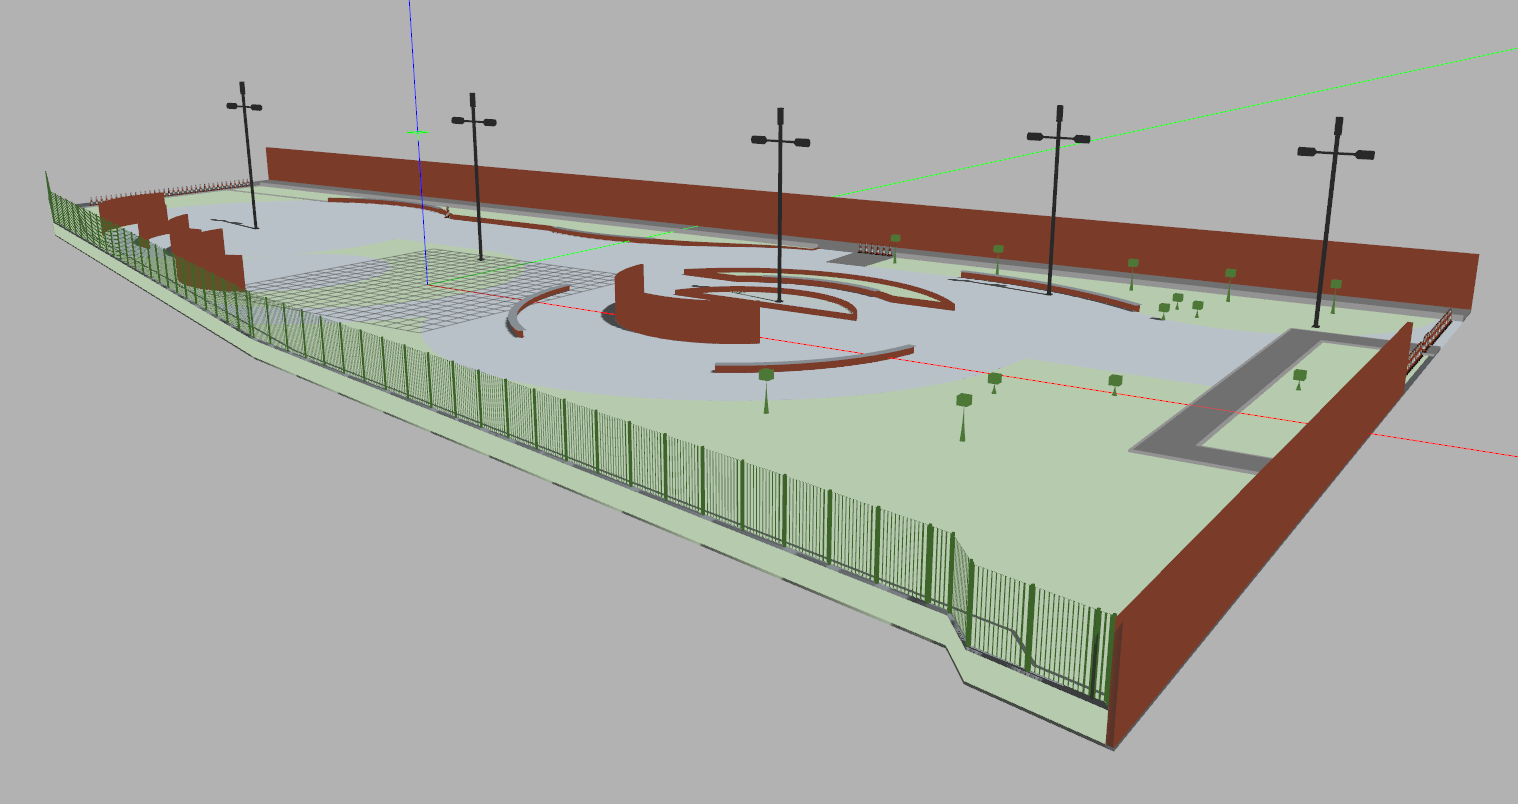
\includegraphics[width= \textwidth]{Figures/cimatec4.png}
    %\caption*{Fonte: Grupo de Formação em Robótica e Sistemas Autônomos}
    %\label{fig:cimatec3_4}
%\end{figure}



\section{Relatório Parcial do Manipulador TIMON-HM- Desafio 2.0 }
\label{sec:desafio_2}
Este desafio está disponível no repositório \url{https://github.com/Brazilian-Institute-of-Robotics/TIMON\_hm\_manipulator}, onde neste também tem os pré-requisitos e o tutorial de como executar a simulação. Na Figura \ref{fig:manipulador_simulacao} é possível verificar o manipulador robótico TIMON-HM no ambiente de simulação do \textit{Gazebo}. No apêndice encontra-se o relatório elaborado para esse desafio, com todas as especificações do mesmo, o estado da arte, metodologia e materiais utilizados.

\begin{figure}[H]
    \caption{Realização do desafio no ambiente de simulação do \textit{Gazebo}}
    \centering
    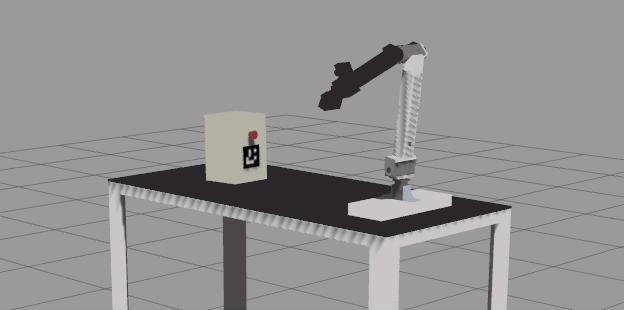
\includegraphics[width= \textwidth]{Figures/manipulador_simulacao.png}
    \caption*{Fonte: Grupo de Formação em Robótica e Sistemas Autônomos}
    \label{fig:manipulador_simulacao}
\end{figure}



\section{Resultado do Manipulador Robótico JeRoTIMON- Desafio 2.2 }
\label{sec:desafio_2_2}
Este desafio está no mesmo repositório \url{https://github.com/Brazilian-Institute-of-Robotics/TIMON\_hm\_manipulator} onde tem a simulação, há também uma parte reservada para o a utilização em ambiente real. Na Figura \ref{fig:manipulador_real} é demonstrado o manipulador JeRoTIMON real e a caixa, e o mesmo executando a missão de pressionar o botão. O relatório elaborado para esse desafio, é o mesmo do \ref{sec:desafio_2}, onde é possível encontrar maiores detalhes do projeto real.



\begin{figure}[H]
    \caption{Realização do desafio no ambiente real}
    \centering
    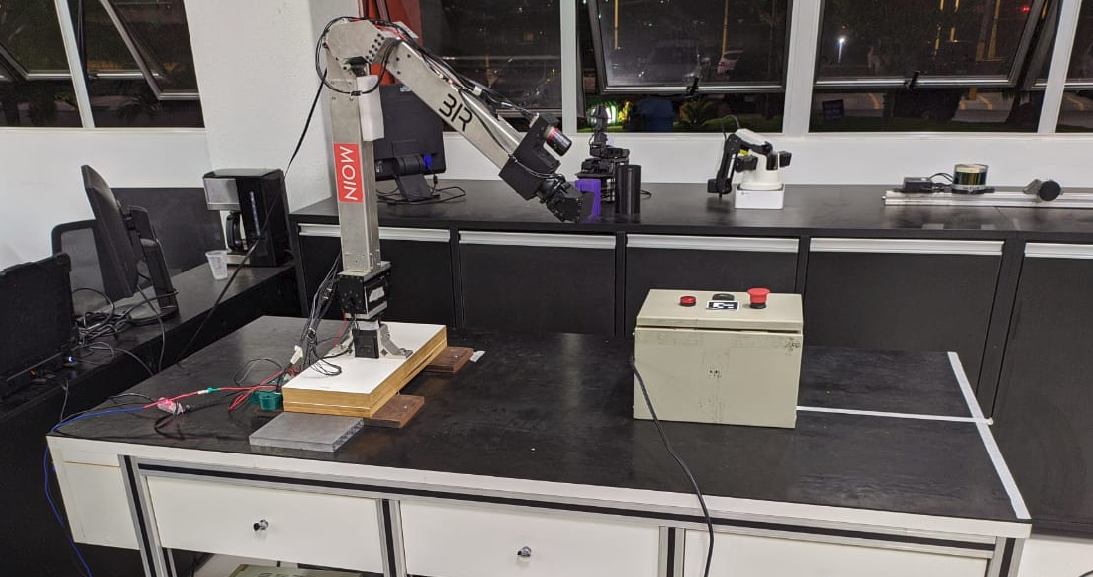
\includegraphics[width= \textwidth]{Figures/manipulador_real.png}
    \caption*{Fonte: Grupo de Formação em Robótica e Sistemas Autônomos}
    \label{fig:manipulador_real}
\end{figure}



\section{TIMON- HM- Desafio 2.5}
\label{sec:desafio_2_5}
O desafio 2.5, disponível no repositório \url{https://github.com/Brazilian-Institute-of-Robotics/TIMON_hm-2-5} onde contam os códigos, pré-requisitos e tutorial para instalação e execução das simulações. Na Figura \ref{fig:marcha_darwinop} tem-se os robôs executando a programação da marcha, e na Figura \ref{fig:revezamento_darwinop} tem-se os robôs executando o código do revezamento.



\begin{figure}[H]
    \caption{Simulação do Desafio 2.5- Marcha}
    \centering
    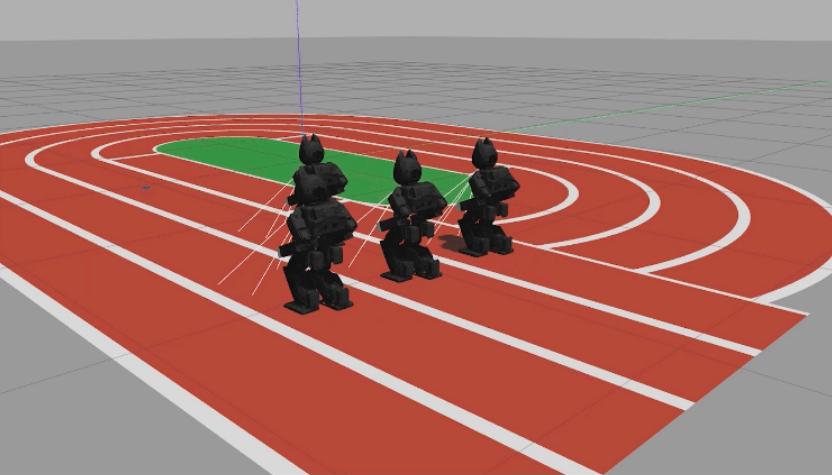
\includegraphics[width= \textwidth]{Figures/marcha.png}
    \caption*{Fonte: Grupo de Formação em Robótica e Sistemas Autônomos}
    \label{fig:marcha_darwinop}
\end{figure}



\begin{figure}[H]
    \caption{Simulação do Desafio 2.5- Revezamento}
    \centering
    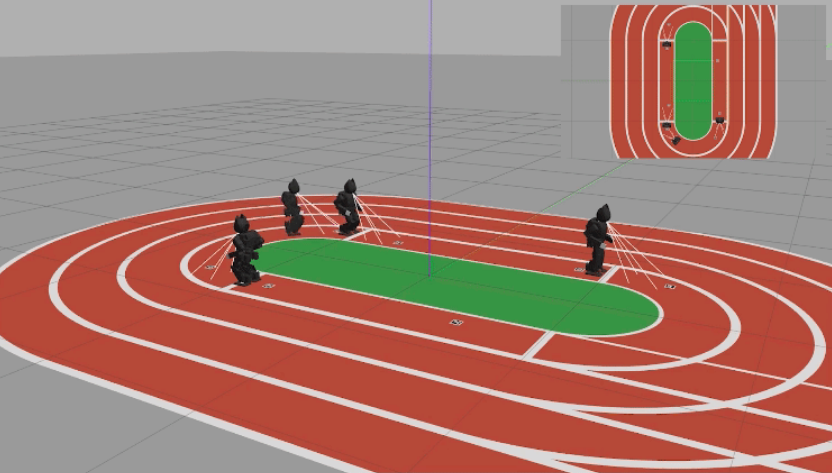
\includegraphics[width= \textwidth]{Figures/revezamento.png}
    \caption*{Fonte: Grupo de Formação em Robótica e Sistemas Autônomos}
    \label{fig:revezamento_darwinop}
\end{figure}

\section{UGV SACI: Integrado com Detecção Visual e Manipulador- Desafio 3.0}
\label{sec:desafio_3_0}
Como resultado obtido desse projeto é possível ver nas Figuras \ref{fig:ambiente_saci}, \ref{fig:warthog_simulacao} e \ref{fig:warthog_desafio_3}, respectivamente, o ambiente externo modelado na simulação, o robô no ambiente de simulação e este no ambiente real.


\begin{figure}[H]
    \caption{Ambiente entre os prédios do CIMATEC 3 e 4 na simulação do \textit{Gazebo}}
    \centering
    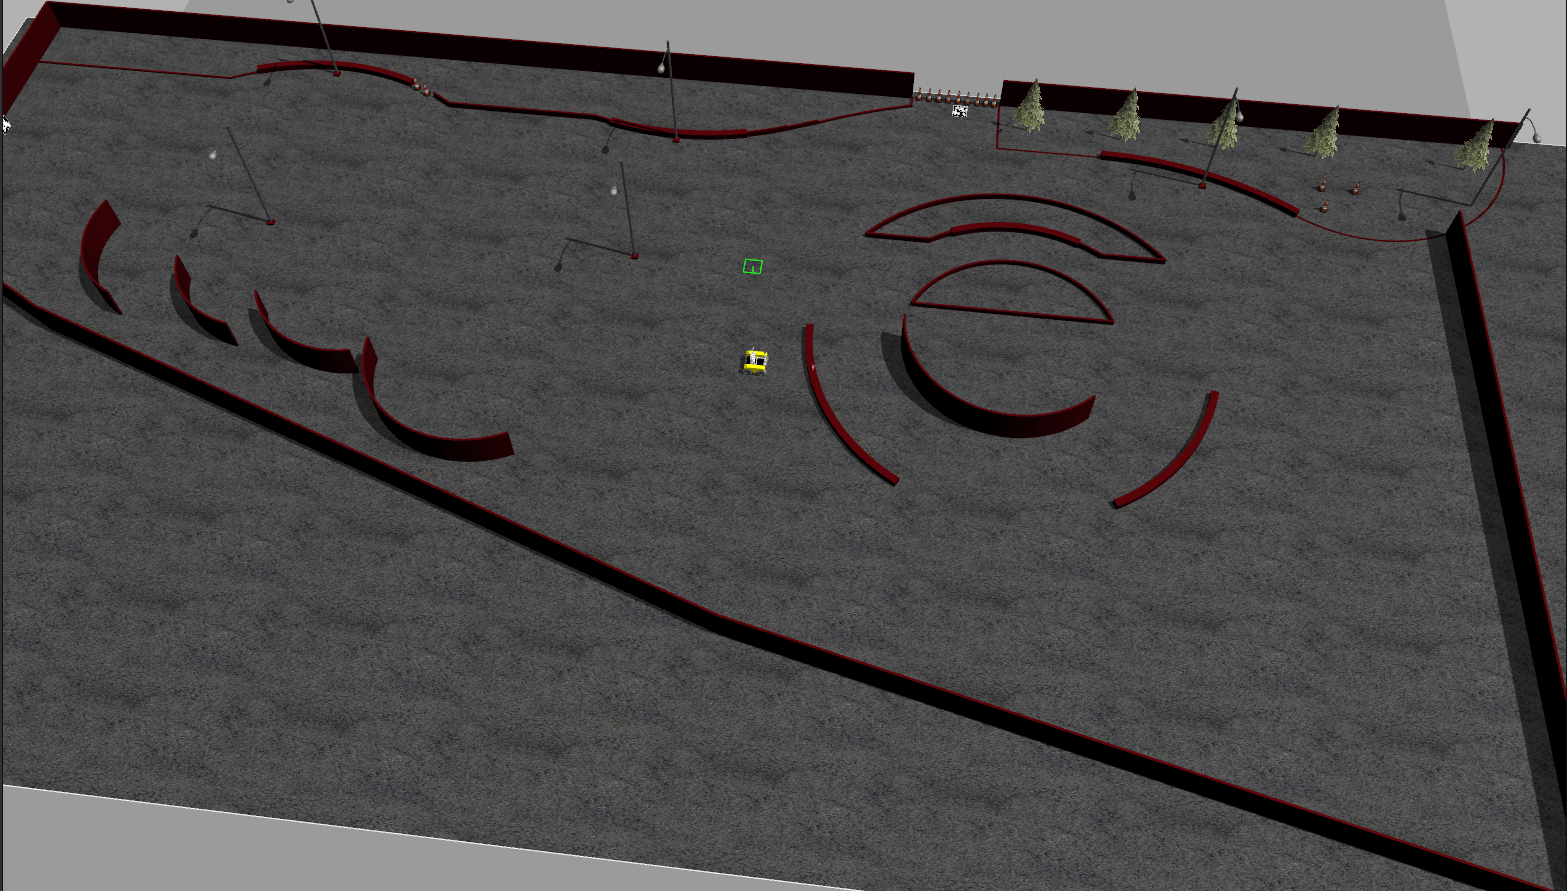
\includegraphics[width= \textwidth]{Figures/ambiente_saci.png}
    \caption*{Fonte: Grupo de Formação em Robótica e Sistemas Autônomos}
    \label{fig:ambiente_saci}
\end{figure}



\begin{figure}[H]
    \caption{Saci modelado para simulação no \textit{Gazebo}}
    \centering
    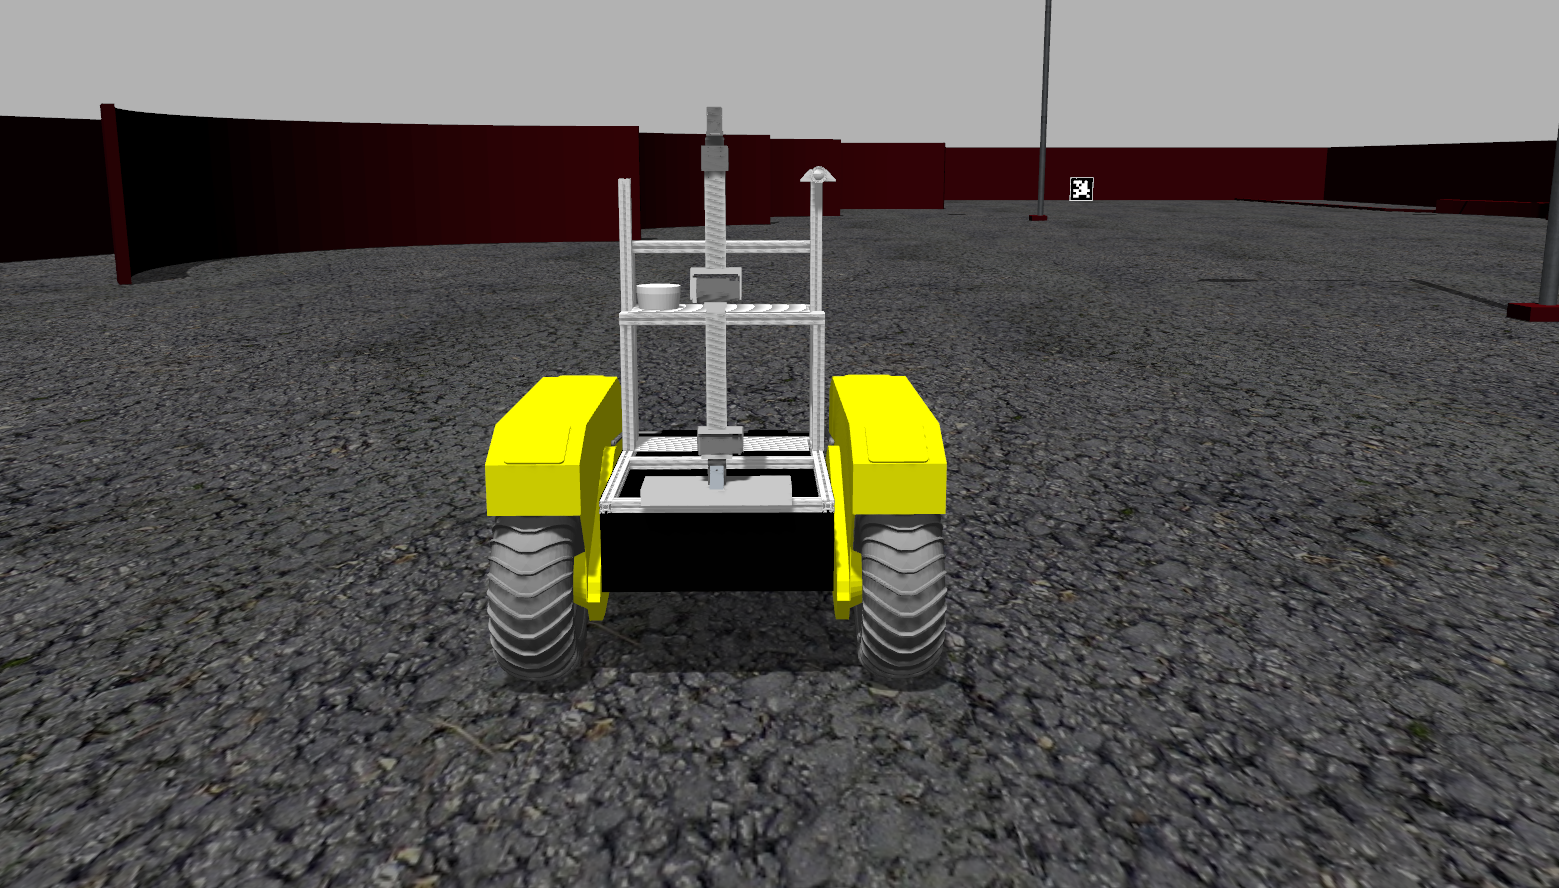
\includegraphics[width= \textwidth]{Figures/warthog_simulacao.png}
    \caption*{Fonte: Grupo de Formação em Robótica e Sistemas Autônomos}
    \label{fig:warthog_simulacao}
\end{figure}


\begin{figure}[H]
    \caption{Modelo Real do Saci, com a identificação dos equipamentos integrados que foram utilizados}
    \centering
    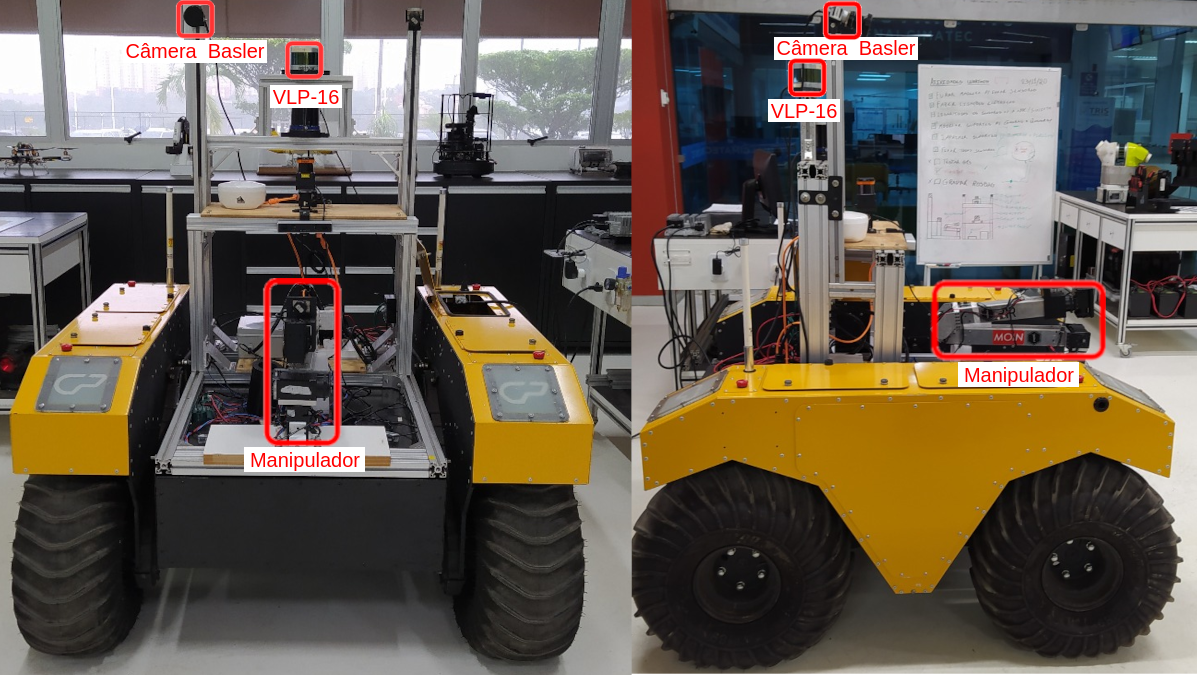
\includegraphics[width= \textwidth]{Figures/warthog_compo2.png}
    \caption*{Fonte: Grupo de Formação em Robótica e Sistemas Autônomos}
    \label{fig:warthog_desafio_3}
\end{figure}


\section{Analíse estatística R\&R da simulação do robô Darwin OP }
\label{sec:analise_darwin}
O resultado proveniente deste estudo está descrito no documento Avaliação do Sistema de Medição- TIMON 2.5 no Apêndices. Onde estão expostos dos dados coletados e a interpretação dos resultados obtidos.


\section{Planejamento de Experimentos (DOE) -Helicóptero de Papel (TIMON-HM)}
\label{sec:analise_doe}
Esse estudo resultou no relatório Planejamento de Experimentos (DOE) -Helicóptero de Papel (TIMON-HM) disponível nos Apêndices, onde neste consta informações sobre o que é o \textit{DOE}, como e qual o motivo da escolha dos fatores de influência e os níveis e os resultados obtidos. 

\section{Resultado do Artigo Manipulador Robótico TIMON-HM- Evento SAPCT 2020 }
\label{sec:sapct}
Para o evento V Seminário de Avaliação de Pesquisa Científica e Tecnológica (SAPCT) e IV Workshop de Integração e Capacitação em Processamento de Alto Desempenho (ICPAD), foi realizado o artigo Projeto e Simulação de um Manipulador Robótico com 5 Graus de Liberdade e Sistema de Visão Integrado, com base no projeto do manipulador robótico TIMON-HM, este artigo consta nos Apêndices, bem como o certificado de participação neste evento.


\section{Resultado do Artigo publicado TRIS: Thermal Remote Identification System of Feverish People- Evento SIINTEC 2020 }
\label{sec:siintec}
O resultado obtido do projeto do \textit{TRIS} foi o artigo publicado no evento VI International Symposium on Innovation and Technology (SIINTEC) 2020, e posteriormente sua premiação em primeiro lugar dentre os trabalhos apresentados. Este artigo TRIS: Thermal Remote Identification System of Feverish People consta nos Apêndices, assim como o certificado de participação nestes evento.